%-----------------------------------------------------------------------------%
\chapter{\babDua}
%-----------------------------------------------------------------------------%

%-----------------------------------------------------------------------------%
\section{Kajian Penelitian Terkait}
%-----------------------------------------------------------------------------%
Banyak sekali referensi yang menjadi bagian besar dalam tertulisnya proposal ini, referensi tersebut terdiri atas berbagai macam jenis literatur dari sumber yang dapat diakses secara daring. Tak sedikit pula literatur tersebut menjadi alasan besar latar belakang dari proposal ini dilahirkan, berikut adalah beberapa penelitian terdahulu yang menjadi referensi dalam melakukan penyusunan proposal ini :

%-----------------------------------------------------------------------------%
% Penelitian Terdahulu
%-----------------------------------------------------------------------------%
\begin{center}			% no	nama	 judul	jurnal		deskripsi
	\begin{longtable}{|p{0.5cm}|p{2cm}|p{3cm}|p{2.5cm}|p{3cm}|}
	\caption{Penelitian Terkait}
	\label{tab:PenelitianDulu}\\
	\hline
	\textbf{No.} & \textbf{Nama} & \textbf{Judul} &\textbf{Jurnal} & \textbf{Deskripsi}\\
	\hline
	1.& Lenz, Isabella;\newline Holtom, Jacob;\newline Herschfelt, Andrew;\newline Rong, Yu;\newline Bliss, Daniel 
	& \textit{Respiratory and Heart Rate Detection Using Continuous-Wave Radar Testbed Implemented in GNU Radio } (2022) \cite{Lenz2022}
	& \textit{Proceedings of the 12th GNU Radio Conference}
	& Penggunaan radar CW untuk observasi detak jantung dan pernapasan menggunakan GNURadio dan USRP X310. Proses pengolahan data secara langsung dengan hasil estimasi pada jarak 5 BPM dibanding alat monitor detak jantung. 
	\\ \hline
	2. 	& Wankhede, Animesh;\newline De, Sampurna
	& \textit{Development of L-Band FMCW Radar on SDR using}
	& \textit{2024 Second International Conference on Emerging Trends in}
	& Penggunaan radar FMCW pada pita frekuensi kelas L \\
	&	
	&\textit{ GNU RADIO} (2024) \cite{Wankhede2024}
	& \textit{Information Technology and Engineering (ICETITE)} 
	&  untuk radar penembus tanah menunjukkan hasil yang efektif dalam melakukan deteksi dan \textit{imaging} objek dengan akurasi dan resolusi tinggi. 
	
	\\ \hline
	
	3. & Hilario Re, Pascual D.;\newline Comite, Davide;\newline Podilchak, Symon K.;\newline Alistarh, Cristian A.;\newline Goussetis, George;\newline Sellathurai, Mathini;\newline Thompson, John;\newline Lee, Jaesup
	& \textit{FMCW Radar With Enhanced Resolution and Processing Time by Beam Switching} (2021) \cite{HilarioRe2021}
	& \textit{IEEE Open Journal of Antennas and Propagation}
	& Implementasi radar FMCW pada frekuensi kelas K dengan antena \textit{array} dan \textit{beammforming} untuk deteksi arah pada kendaraan otomotif. Radar mampu mendeteksi objek dengan jarak 2\textdegree.
	\\ \hline
	4.& Dabrowski, Grzegorz;\newline Stasiak, Krzysztof;\newline Drozdowicz, Jedrzej;\newline Gromek, Damian;\newline Samczynski, Piotr
	& \textit{An X–band FMCW Radar Demonstrator Based on an SDR Platform} (2020) \cite{Dabrowski2020}
	& \textit{2020 21st International Radar Symposium (IRS)}
	& Desain radar FMCW dengan \textit{bandwidth} 1 GHz untuk mendapatkan resolusi jarak yang kecil, didapat hasil pengujian \\
	&
	&
	&
	& yang memuaskan dengan adanya pergerakan pada daerah yang ditandai memiliki banyak aktivitas. \\ \hline
	
	5.& Rizik, Ali;\newline Tavanti, Emanuele;\newline Vio, Roberto;\newline Delucchi, Alessandro;\newline Chible, Hussien;\newline Randazzo, Andrea;\newline Caviglia, Daniele D.
	& \textit{Single Target Recognition Using a Low-Cost FMCW Radar Based on Spectrum Analysis} (2020) \cite{Rizik2020}
	& \textit{2020 27th IEEE International Conference on Electronics, Circuits and Systems (ICECS)}
	& Pengolahan sinyal radar dilakukan dengan klasifikasi data menggunakan \textit{Support Vector Machine} (SVM), didapat hasil menunjukkan akurasi klasifikasi target mencapai 100\%. 
	\\ \hline
	6. & Jeong, Hyunmin;\newline Kim, Sangkil
	& \textit{Educational Low-Cost C-Band FMCW Radar System Comprising Commercial} 
	& \textit{Electronics}
	& Desain dan implementasi radar FMCW pada frekuensi kelas C dilakukan menggunakan \\
	&
	&\textit{ Off-the-Shelf Components for Indoor Through-Wall Object Detection} (2021) \cite{Jeong2021}
	& 
	& komponen elektronik yang mudah didapat. Implementasi dilakukan dengan skenario pengujian dalam ruangan dan tembus dinding. Didapat hasil rata rata akurasi sekitar 5.6 cm. \\ \hline
	
	7. & Pramudita, Aloysius Adya;\newline Suratman, Fiky Y.;\newline Arseno, Dharu
	& \textit{Modified FMCW system for non-contact sensing of human respiration} (2020) \cite{Pramudita2020}
	& \textit{Journal of Medical Engineering and Technology}
	& Dengan melakukan modifikasi pada pengolahan data fasa setelah filter \textit{Low Pass}. Didapatkan hasil bahwa desain\\
	&
	&
	&
	&
	 modifikasi mampu mendeteksi waktu dan amplitudo pernafasan, serta lokasi dari target. 
	\\
	\hline
	8. & Pramudita, Aloysius Adya;\newline Lin, Ding-Bing;\newline Dhiyani, Azizka Ayu;
	& \textit{FMCW Radar for Noncontact Bridge Structure Displacement Estimation} (2023) \cite{Pramudita2023}
	& \textit{IEEE Transactions on Instrumentation and Measurement}
	& Implementasi radar FMCW pada frekuensi 24 GHz dengan \textit{bandwidth} 150 MHz untuk mendeteksi \\
	& Ryanu, Harfan Hian;\newline Adiprabowo, Tjahjo;\newline Yudha, Erfansyah Ali
	&
	&
	&
	pergeseran kecil pada bangunan jembatan. Hasil menunjukkan metode berhasil dengan kondisi banyak \textit{noise} dan nilai SNR rendah dengan rata rata galat 0.13 mm.
	\\ \hline
	9. & Zhou, Min;\newline Liu, Yunxue;\newline Wu, Shie;\newline Wang, Chengyou;\newline Chen, Zekun;\newline Li, Hongfei
	& \textit{A Novel Scheme of High-Precision Heart Rate Detection With a mm-Wave FMCW Radar} (2023) \cite{Zhou2023}
	& \textit{IEEE Access}
	& Radar FMCW dengan gelombang milimeter untuk peningkatan akurasi menggunakan algoritma \textit{Variable Mode Extraction} dan teknik pengukuran \\
	&
	&
	&
	&
	frekuensi \textit{Double-CZT}. Tingkat akurasi meningkat dengan rata rata eror absolut kurang dari 1 bpm, nilai SNR meningkat sehingga estimasi akurasi detak jantung juga meningkat.
	\\ \hline
	\end{longtable}
\end{center}

Pada penelitian \cite{Lenz2022}, menunjukkan teknik yang perlu dilakukan saat melakukan pengolahan data hasil radar secara \textit{real time} yaitu dengan menggunakan ZeroMQ yang dapat mengirimkan data dari aplikasi satu ke lainnya, sehingga pengolahan bisa dilakukan dengan pemrograman berbahasa \textit{python}. Penelitian \cite{Wankhede2024} menunjukkan referensi parameter radar FMCW yang dapat diraih oleh USRP menggunakan GNURadio. Penelitian \cite{HilarioRe2021} menunjukkan kemampuan radar FMCW bila dilakukan implementasi dengan menggunakan antena \textit{array} untuk mendeteksi arah datang suatu objek.

Penelitian \cite{Dabrowski2020} menunjukkan skenario yang harus dilakukan dalam melakukan pengujian bila jarak radar didapat sangat jauh, sehingga perlu beberapa teknik pengujian yang dilakukan untuk mengambil keputusan dan menilai radar yang telah didesain. Penelitian \cite{Rizik2020} memperlihatkan kapabilitas radar bila dilakukannya analisa data lebih lanjut, yaitu dalam mengklasifikasikan data antara orang berjalan kaki dan kendaraan. Penelitian \cite{Jeong2021} menunjukkan langkah yang perlu dilakukan dalam merancang analisa hasil radar dan membandingkannya dengan nilai ekspektasi.

Penelitian \cite{Pramudita2020} menggunakan analisa pada fasa untuk memperoleh data yang diinginkan, hal ini menunjukkan titik observasi lain masih dapat dilakukan untuk mendapatkan data yang diinginkan bila hasil tidak sesuai dengan ekspektasi. Penelitian \cite{Pramudita2023} menunjukkan teknik pengujian dan analisa yang perlu dilakukan dalam melakukan pengujian radar FMCW, hingga perbandingan antara radar yang didesain dengan radar komersial untuk menentukan kualitas radar yang dirancang. Penelitian \cite{Zhou2023} memperlihatkan bahwa teknik analisa hasil tidak hanya dapat dilakukan dengan FFT, namun algoritma lain dapat dilakukan sehingga estimasi akan semakin akurat.

%-----------------------------------------------------------------------------%
%\section{Teori Dasar}
%-----------------------------------------------------------------------------%

\section{Radar}

Penggunaan gelombang elektromagnetik sebagai sarana untuk mendeteksi objek adalah konsep dasar dari radar. Radar sendiri merupakan singkatan dari \textit{Radio Detection and Ranging}, dari situ sangat nampak sekali tujuan dari penggunaan alat ini, yaitu untuk mendeteksi sesuatu dan mengukur jarak dengan menggunakan gelombang radio. 

Cara kerja dari radar adalah dengan memancarkan gelombang di dalam ruang bebas yang kemudian radar akan mendeteksi gelombang pantulan dari objek tersebut. Adanya gelombang yang terpantul ini tidak hanya menunjukkan keberadaan dari suatu objek, namun dengan membandingkan gelombang pantulan yang diterima dengan gelombang yang dikirimkan maka informasi tentang objek yang terdeteksi dapat dihitung \cite{Skolnik2001}. 

\begin{equation}
	R = \frac{cT_{R}}{2}
	\label{eq:PersRadar}
\end{equation}

Persamaan~(\ref{eq:PersRadar}) menjelaskan jarak antara target dengan antena yang disimbolkan sebagai $R$ (meter), dengan $T_{R}$ (sekon) sebagai waktu sinyal radar bergerak secara bolak balik dari dan menuju objek. Karena radar memakai gelombang elektromagnetik, maka $c$ memiliki kecepatan yang sama dengan cahaya, yaitu $3 \cdot 10 ^{8} $ m/s.

\begin{figure}
	\begin{center}
		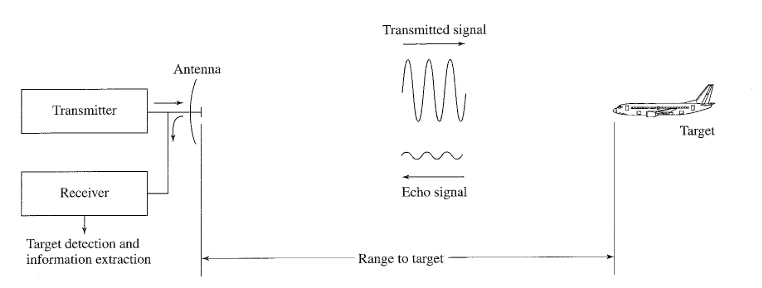
\includegraphics[scale=0.3]{pics/bab2/skemaradar.png} 
		\caption[Skema Dasar Radar]{{Skema Dasar Radar} \cite{Skolnik2001}}
		\label{pic:skemaRadar}
	\end{center}
\end{figure}

Pada gambar \ref{pic:skemaRadar}, skema dan konsep dasar dari cara kerja radar dapat diamati. Terlihat bahwa sinyal yang dikirimkan akan mengenai target, dalam kasus ini adalah pesawat, lalu sinyal yang mengenai objek akan kembali dengan sinyal yang lebih kecil dengan amplitudo yang lebih rendah. Perubahan pada gelombang yang terpantul dapat menggambarkan perilaku yang sedang ditunjukkan oleh objek yang di deteksi, mulai dari pengurangan amplitudo hingga pergeseran fasa.

\begin{figure}
	\begin{center}
		\includegraphics[scale=0.32]{pics/bab2/blokdiagram.png} 
		\caption[Blok Diagram Radar]{{Blok Diagram Radar Sederhana \cite{Kingsley1999}}}
		\label{pic:blokdiagram}
	\end{center}
\end{figure}

Gambar \ref{pic:blokdiagram} menunjukkan blok diagram dari sistem radar pulsa sederhana. Dapat dilihat beberapa komponen yang membentuk seluruh sistem radar, semua komponen ini memiliki perannya sendiri sehingga proses pengiriman dan pendeteksian sinyal dapat dilakukan.  Bila seluruh sistem bekerja dengan baik, maka proses yang ditunjukkan pada penjelasan skema dasar radar dapat berjalan dengan lancar.

Persamaan radar berguna untuk menghubungkan seluruh komponen yang terdapat pada suatu sistem radar. Hubungan di antara seluruh komponen tersebut akan di perlihatkan secara matematis, sehingga penerapannya pada suatu alat akan terlihat dengan jelas. Dengan adanya beberapa persamaan ini, proses desain suatu radar akan menjadi lebih mudah dilakukan dan prediksi dari hasil radar yang dirancang bisa didapatkan.

\begin{equation}
	R_{un} = \frac{cT_{p}}{2} = \frac{c}{2f_{p}}
	\label{eq:maxUnRan}
\end{equation}

Salah satu persamaan pada radar adalah \textit{maximum unambiguous range} menunjukkan jarak tempuh radar terjauh yang dapat dideteksi disimbolkan sebagai $R_{un}$ (meter) pada persamaan~(\ref{eq:maxUnRan}), dengan $c$ adalah kecepatan cahaya, $T_{p}$ sebagai periode pengulangan pulsa yang biasa menggunakan satuan sekon bahkan mikrosekon, dan $f_{p}$ sebagai frekuensi pengulangan pulsa (Hz). Sehingga $T_{p}$ berbanding terbalik dengan $f_{p}$.

\begin{equation}
	T_{p} = \frac{1}{f_{p}}
	\label{eq:pulseFreq}
\end{equation}

Persamaan~(\ref{eq:pulseFreq}) menunjukkan hubungan periode pengulangan pulsa radar ($T_{p}$) dengan frekuensi pengulanganya ($f_{p}$). Semakin besar frekuensi pengulangan pulsa radar, maka periode pengulanganya akan semakin kecil.

\begin{equation}
	P = \frac{P_{t}}{4\pi R^{2}}
	\label{eq:powIso}
\end{equation}

Bila antena yang digunakan dalam memancarkan gelombang elektromagnetika radar bersifat isotrop, maka kerapatan daya pada jarak $R$ dari radar akan sama dengan daya dalam satuan Watt di transmisi ($P_{t}$) dibagi luas permukaan $4\pi R^{2}$ dari sebuah bola imajiner dengan radius $R$ (meter), atau dapat didefinisikan pula dengan persamaan~(\ref{eq:powIso}), namun kenyataannya tidak seperti itu.

\begin{equation}
	\text{Kerapatan daya antena \textit{directional}} = \frac{P_{t} G}{4\pi R^{2}}
	\label{eq:powDir}
\end{equation}

Radar seringkali menggunakan antena \textit{directive} untuk mengkonsentrasikan daya yang terradiasi pada arah tertentu. Maka kerapatan dayanya seperti pada persamaan~(\ref{eq:powDir}), dengan G sebagai \textit{gain} maksimum suatu antena yang terdefinisi sebagai berikut.

\begin{equation}
	G  = \frac{\text{Kerapatan daya maksimum dari antena \textit{directional}}}{\text{Kerapatan daya antena Isotrop \textit{lossless} dengan daya yang sama}}
\end{equation}

\textit{Gain} bersatuan dB (desibel) yang menunjukkan perbandingan suatu nilai, dalam kasus ini kerapatan daya maksimum antena berarah dibanding antena isotropik.

\section{Pengolahan Sinyal Radar}
Untuk mendapat suatu kesimpulan dari sinyal radar, maka dibutuhkan pengolahan sinyal radar yang tepat. Pengolahan sinyal tersebut dilakukan mulai dari pembentukan gelombang hingga pengambilan kesimpulan. 

\subsection{Bentuk Gelombang Radar}

Bentuk gelombang radar dapat dibedakan menjadi dua kelas, yaitu radar dengan gelombang kontinyu dan radar pulsa. Seperti pada gambar \ref{pic:bentukgelradar}, kedua kelas tersebut masih dapat dibagi lagi kedalam beberapa teknik lain. Penggunaan salah satu jenis gelombang ditentukan berdasarkan kebutuhan radar yang akan di desain. 

\begin{figure}
	\begin{center}
		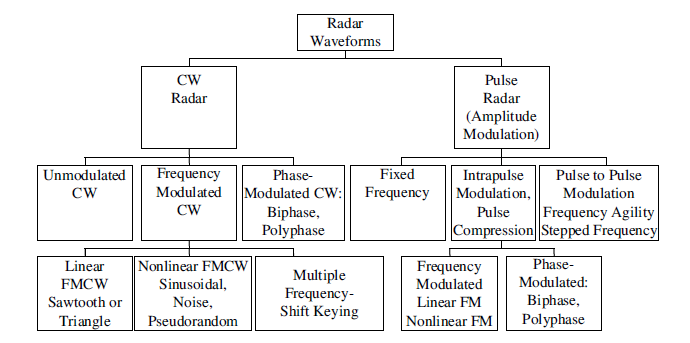
\includegraphics[scale=0.8]{pics/bab2/radarwaveform.png}
		\caption[Bentuk Gelombang Radar]{Bentuk Gelombang Radar \cite{Melvin2014}}
		\label{pic:bentukgelradar}
	\end{center}
\end{figure}


Radar dengan gelombang pulsa akan memancarkan gelombang elektromagnetik dalam waktu singkat lalu jeda sejenak sesuai waktu yang ditentukan. Pada waktu jeda tersebut, radar akan mendeteksi sinyal pantul dari gelombang yang dikirim sebelumnya. Setelah waktu jeda berakhir, radar akan kembali memancarkan gelombang pulsa lagi. Radar dengan gelombang ini akan memancarkan gelombang elektromagnetik dengan \textit{power} yang tinggi. 

Sedangkan radar dengan gelombang kontinyu akan terus memancarkan serta menerima gelombang elektromagnetik tanpa henti dalam waktu yang bersamaan. Sehingga radar dengan gelombang kontinyu hanya digunakan pada sistem dengan \textit{power} yang rendah dengan jarak maksimum deteksi yang kecil. Hal ini disebabkan karena sering terjadinya kebocoran dari antena pengirim ke antena penerima. Alasan ini pula yang mendasari keputusan penggunaan \textit{power} yang rendah \cite{Scheer2015}.

\subsection{\textit{Frequency Modulated Continuous Wave Radar}}

Radar FMCW memancarkan sinyal yang bila terpantul objek, akan kembali terdeteksi. Hal ini dapat direalisasikan dengan blok diagram dari sistem radar FMCW seperti pada gambar \ref{pic:FMCWBlock}.  

\begin{figure}
	\begin{center}
		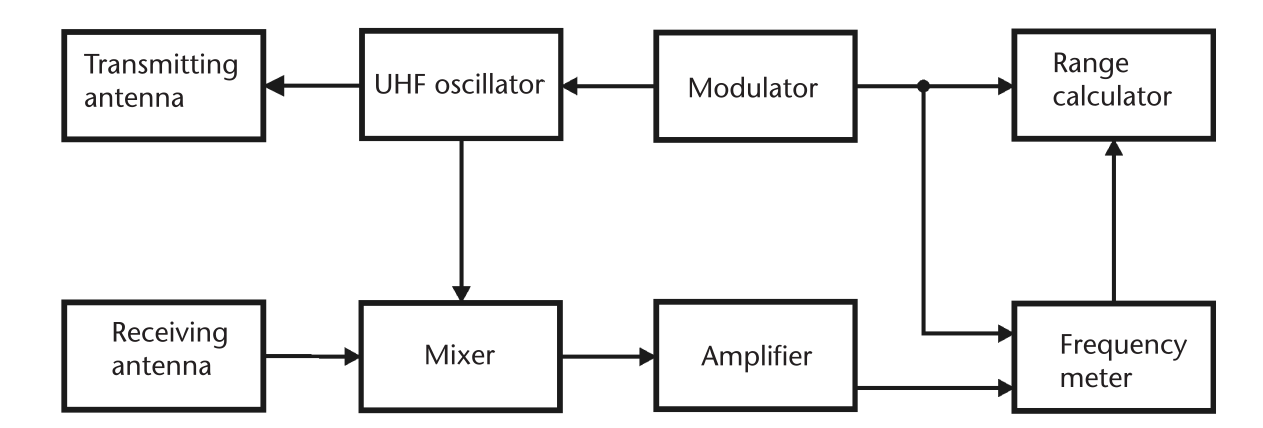
\includegraphics[scale=0.3]{pics/bab2/blokDiagramFMCW.png}
		\caption[Blok Diagram Radar FMCW]{Blok Diagram Radar FMCW}
		\label{pic:FMCWBlock}
	\end{center}
\end{figure}

Dari blok diagram tersebut, dapat dilihat bahwa sinyal yang diterima akan dicampurkan dengan sinyal yang dikirim, bila terdapat \textit{delay} yang disebabkan oleh jarak, maka akan terdeteksi perbedaan frekuensi. Dengan begitu, perbedaan pada fasa dan frekuensi menjadi tolok ukur antara sinyal yang dikirim dengan sinyal yang di dapatkan kembali.

\begin{figure}
	\begin{center}
		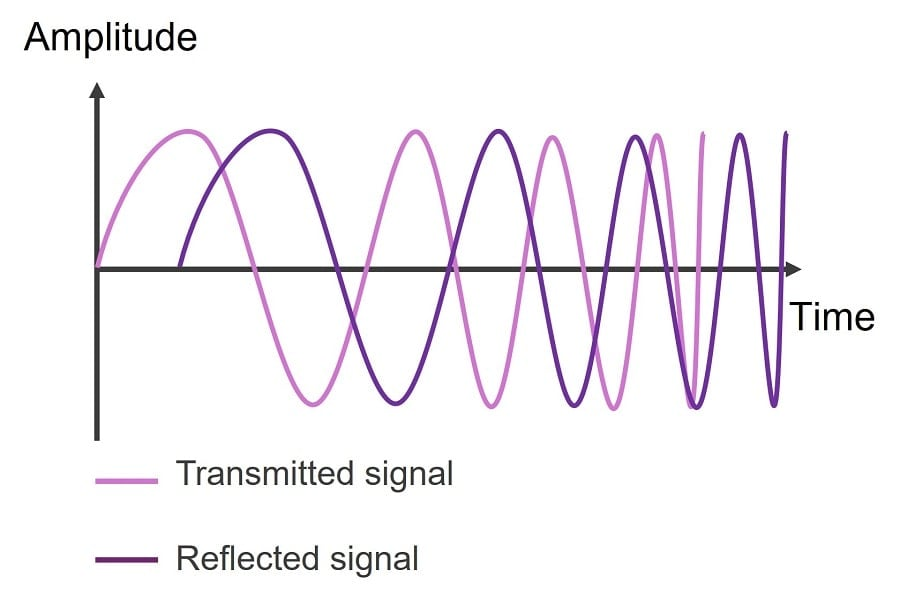
\includegraphics[scale=0.4]{pics/bab2/txRxWave.jpg}
		\caption[FMCW Dalam Domain Waktu]{FMCW Dalam Domain Waktu}
		\label{pic:FMCWTime}
	\end{center}
\end{figure}

Oleh karena itu, salah satu karakteristik dari radar FMCW adalah bahwa jarak pengukuran dapat dihitung dengan membandingkan frekuensi sinyal yang diterima dengan sinyal yang ditransmisikan seperti pada gambar \ref{pic:FMCWTime}.   

\begin{equation} 
	R = \frac{c \Delta{t}}{2} = \frac{c \Delta{f}}{2(\frac{d(f)}{d(t)})}
	\label{eq:PersFMCW}
\end{equation}

Persamaan~(\ref{eq:PersFMCW}) menunjukkan jarak (R) dalam meter dengan objek yang terdeteksi. Yang mana $\Delta{t}$ adalah waktu tunda dalam detik, $\Delta{f}$ merupakan pergeseran frekuensi terukur dalam Hertz, dengan d(f)/d(t) sebagai pergeseran frekuensi dalam suatu periode. 

\begin{equation}
	R_{max} = \frac{F_{s} c}{2 \mu}
	\label{eq:MaxRange}
\end{equation}

Persamaan~(\ref{eq:MaxRange}) menunjukkan jarak maksimum yang dapat di deteksi oleh radar FMCW. $F_{s}$ merupakan frekuensi \textit{sampling} yang biasanya menggunakan satuan Hertz atau \textit{Sample/second}, dan $\mu$ adalah tingkat kenaikan frekuensi pada suatu periode disimbolkan dengan Hertz/sekon.

\begin{equation}
	\mu = \frac{\textit{Bandwidth}}{T_{c}}
	\label{eq:chirpRate}
\end{equation}

Persamaan~(\ref{eq:chirpRate}) adalah langkah menghitung $\mu$ yaitu membagi nilai \textit{bandwidth} dengan waktu \textit{sweep} (\textit{chirp}) bersimbol $T_{c}$. Biasanya, radar FMCW memiliki nilai $T_{c}$ yang kecil, dengan menggunakan satuan $\mu s$, sehingga nilai \textit{chirp rate} memiliki satuan $Hz/\mu s$

\begin{equation}
	T_{c} = \frac{\lambda}{4 \cdot V_{max}}
	\label{eq:chirpTime}
\end{equation}

Dengan nilai $T_{c}$ yaitu periode \textit{chirp} didefinisikan sebagai persamaan~(\ref{eq:chirpTime}), dengan $\lambda$ sebagai panjang gelombang (meter) dan $V_{max}$ sebagai kecepatan maksimum yang dapat dideteksi oleh radar (m/s).

Selain itu, salah satu faktor penting yang perlu diperhitungkan dalam perancangan radar FMCW adalah resolusi jarak. Resolusi jarak sendiri merupakan kemampuan dari suatu radar dalam membedakan dua buah objek yang berdekatan.

\begin{equation}
	R_{res} = \frac{c}{2 BW}
	\label{eq:RangeRes}
\end{equation}

Persamaan~(\ref{eq:RangeRes}) menjelaskan bahwa dengan membagi kecepatan cahaya dengan dua kali lebar pita frekuensi (\textit{Bandwidth}) dalam Hertz, maka resolusi jarak dalam satuan meter akan didapatkan. 

\begin{equation}
	v_{max} = \frac{\lambda}{4 \cdot T_{c}}
	\label{eq:maxVelo}
\end{equation}

Nilai kecepatan maksimum dapat dihitung dengan persamaan~(\ref{eq:maxVelo}), yaitu panjang gelombang frekuensi yang digunakan (Hz) dibagi dengan \textit{sweep time} dalam sekon ($T_{c}$) dikalikan empat.

\begin{equation}
	V_{res} = \frac{\lambda}{2 \cdot T_{f}}
	\label{eq:resVelo}
\end{equation}

Sehingga nilai resolusi kecepatan dapat dihitung dengan persamaan~(\ref{eq:resVelo}), yang membagi panjang gelombang (Hz) dengan 2 kali durasi \textit{frame} ($T_{f}$) dalam sekon.

\begin{equation}
	T_{f} = N \cdot T_{c} = \frac{\lambda}{2 \cdot V_{res}}
	\label{eq:frameDuration}
\end{equation}

$T_{f}$ adalah durasi dari \textit{frame} yang terdiri dari N jumlah dari \textit{chirp} secara terus menerus, nilainya dapat dicari pada persamaan~(\ref{eq:frameDuration}).

\subsection{\textit{Linear Frequency Modulated Continuous Wave Radar}}
\textit{Linear Frequency Modulated}, yang juga sering disingkat sebagai LFM adalah teknik pengolahan sinyal yang dilakukan dengan menyapu frekuensi dari bawah ke atas (\textit{Up-Chirp}) atau dari atas ke bawah (\textit{Down-Chirp}). Dengan $f_{0}$ sebagai frekuensi tengah, dan dilakukan pada \textit{bandwidth} yang telah ditentukan. Teknik ini akan membantu pencapaian radar dengan resolusi yang lebih tinggi karena \textit{bandwidth} yang dicapai akan menjadi lebih tinggi.

Salah satu jenis gelombang LFM adalah \textit{Linear Triangular Frequency Modulation} yang ditunjukkan pada gambar \ref{pic:LFMTriangular}. Penggunaan jenis gelombang tersebut akan mempermudah proses evaluasi target. Alasannya adalah saat objek yang terdeteksi bergerak menjauh dari radar, maka frekuensi akan bergeser turun karena \textit{doppler} dan dua \textit{beat frequency} akan muncul, satu pada \textit{upchirp} dan satu pada \textit{downchirp}. 

Saat objek berada pada jarak yang jauh, namun tidak bergerak, maka akan terjadi \textit{beat frequency} akibat kemunduran waktu. Bila keduanya terjadi dalam waktu yang bersamaan, maka dua nilai \textit{beat frequency} akan muncul, sehingga sumber pergeseran frekuensi dapat dibedakan diantara \textit{doppler} dengan \textit{delay} waktu.

\begin{figure}
	\begin{center}
		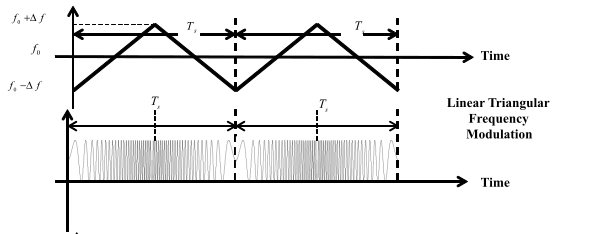
\includegraphics[scale=0.55]{pics/bab2/lfmTriangular.png}
		\caption[LFM Tipe Segitiga]{LFM Tipe Segitiga \cite{Jankiraman2018}}
		\label{pic:LFMTriangular}
	\end{center}
\end{figure}


Selain gelombang LFM segitiga, ada pula yang berbentuk seperti gigi gergaji (\textit{Sawtooth}) seperti gambar \ref{pic:lfmSaw}.

\begin{figure}
	\begin{center}
		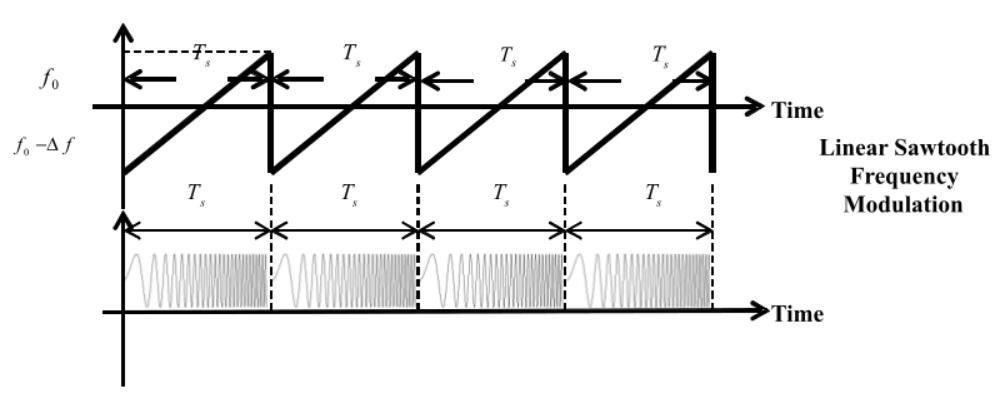
\includegraphics[scale=0.65]{pics/bab2/lfmSawtooth.png}
		\caption[LFM Tipe Gigi Gergaji]{LFM Tipe Gigi Gergaji \cite{Jankiraman2018}}
		\label{pic:lfmSaw}
	\end{center}
\end{figure}

Seluruh teknik tersebut memiliki keunggulannya masing-masing. Keunggulan tersebut didapat karena proses analisis yang berbeda. Pada LFM berbentuk gigi gergaji, maka hanya objek diam saja yang dapat dideteksi jarak dan kecepatannya seperti pada gambar \ref{pic:lfmDetail}.

\begin{figure}
	\begin{center}
		\includegraphics[scale=0.65]{pics/bab2/lfmDetail.png}
		\caption[Detail Analisis LFM \textit{Sawtooth}]{Detail Analisis LFM \textit{Sawtooth} \cite{Jankiraman2018}}
		\label{pic:lfmDetail}
	\end{center}
\end{figure}

Bila menggunakan LFM berbentuk segitiga, maka objek yang bergerak dapat dideteksi jarak dan kecepatannya dalam waktu yang bersamaan. Cara melakukan analisa pada teknik LFM segitiga dapat dilihat lebih jelas pada gambar \ref{pic:DetailMod}.

\begin{figure}
	\begin{center}
		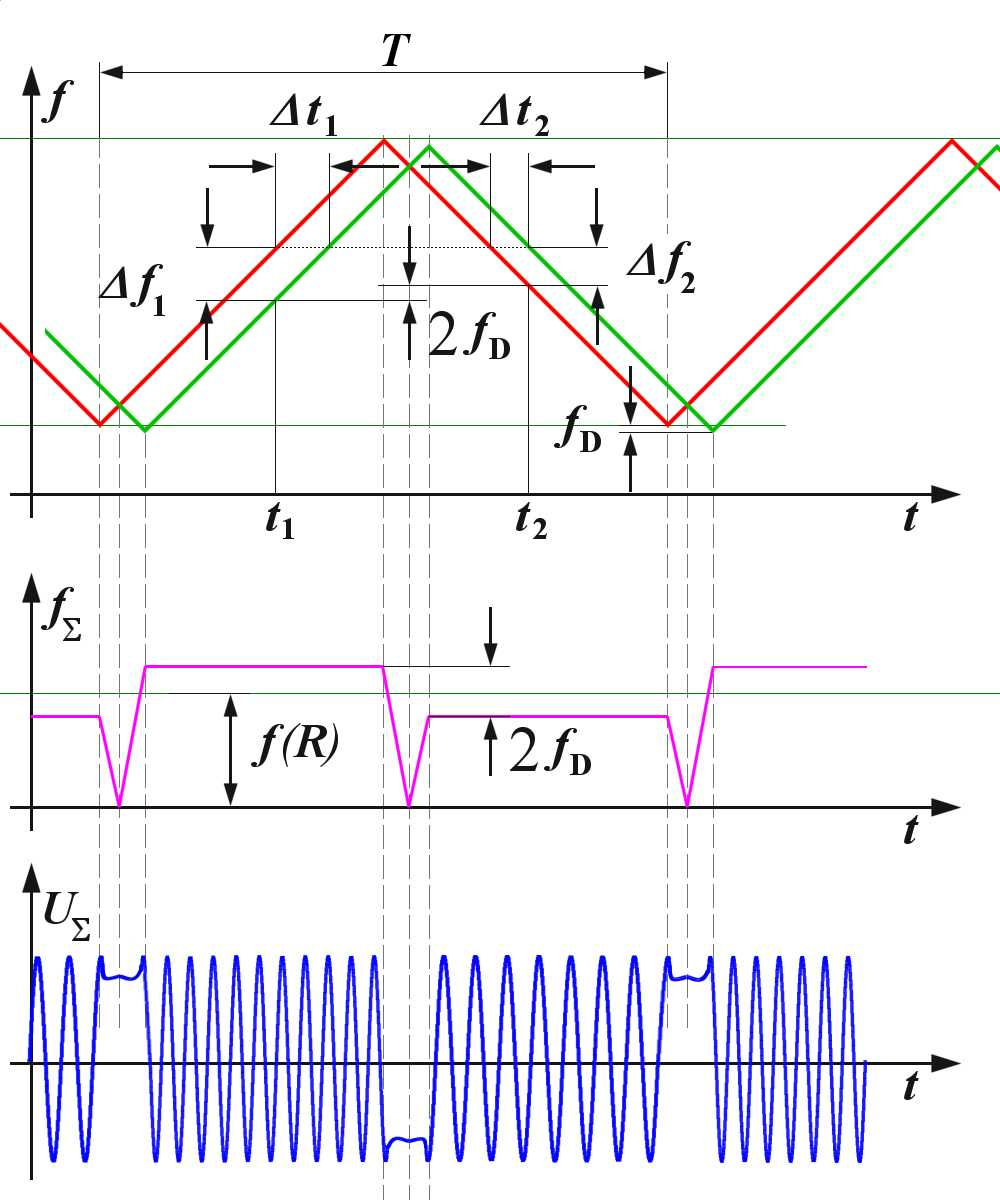
\includegraphics[scale=0.26]{pics/bab2/DetailMod.jpg}
		\caption[Detail Analisa LFM \textit{Triangular}]{Detail Analisis LFM \textit{Triangular}}
		\label{pic:DetailMod}
	\end{center}
\end{figure}

Gambar \ref{pic:DetailMod} menunjukkan langkah analisa gelombang LFM tipe segitiga. $\Delta t$ adalah pergeseran frekuensi akibat kemunduran waktu, sedangkan $\Delta f$ adalah pergeseran frekuensi akibat \textit{doppler}. Dengan T sebagai periode \textit{chirp} yang terjadi pada radar.

\subsection{Teknik Pengolahan Sinyal}
Untuk melakukan pengambilan keputusan dari data yang diambil oleh radar, maka dibutuhkan langkah pengolahan yang benar dan mencakup berbagai hal. Beberapa parameter yang bisa diambil estimasinya adalah jarak dan kecepatan dari objek yang terdeteksi. Pada estimasi jarak, persamaan~(\ref{eq:RangeEst}) dapat menjelaskan hubungan jarak dengan beberapa faktor yang mempengaruhinya.

\begin{equation}
	d_{0} = \frac{c f_{b}}{2 \mu} = \frac{c T_{c} f_{b}}{2 BW}
	\label{eq:RangeEst}
\end{equation}

Pada persamaan~(\ref{eq:RangeEst}) tersebut, $d_{0}$ merujuk ke hasil estimasi jarak dengan satuan meter,  c sebagai kecepatan cahaya, $f_{b}$ adalah \textit{beat frequency} yang merupakan perbedaan pada frekuensi dalam Hertz, $\mu$ yang merupakan laju perubahan frekuensi pada suatu waktu (\textit{chirp rate}) disimbolkan sebagai Hz/s, dengan $T_{c}$ sebagai waktu \textit{Sweep}. Sedangkan untuk melakukan estimasi kecepatan terdapat pergeseran frekuensi akibat efek doppler, yang menjelaskan perubahan frekuensi suatu gelombang karena suatu objek sumber yang bergerak. 

\begin{equation}
	v = \frac{f_{d}}{2}\lambda
	\label{eq:velocity}
\end{equation}

Persamaan~(\ref{eq:velocity}) akan didapat dengan menunjukkan hubungan antara pergeseran doppler ($f_{d}$), dengan v sebagai kecepatan yang memiliki satuan m/s, dan $\lambda$ adalah panjang gelombang dengan satuan meter. 

\subsection{Perhitungan \textit{Error}}
Penghitungan galat dari radar yang telah di desain dapat dilakukan dengan menguji keakurasian dari hasil deteksi. Hasil akurasi deteksi radar dapat diuji dengan menggunakan \textit{Root Mean Square Error} (RMS E). Nilai dari RMS E bisa didapat dengan persamaan~(\ref{eq:rmsE}) dengan nilai n adalah jumlah pengulangan dari uji coba.

\begin{equation}
	RMS E = \sqrt{\frac{\sum_{i = 1}^{n} (simulasi_{i}-aktual_{i})^2}{n}}
	\label{eq:rmsE}
\end{equation}

\section{\textit{Software Defined Radio}}
\textit{Software Defined Radio} atau yang sering disingkat menjadi SDR merupakan teknologi komunikasi berbasis nirkabel yang kegunaannya dapat ditentukan oleh perangkat lunak \cite{Anisah2018}. Sehingga dalam implementasinya, tidak perlu dilakukan perubahan perangkat keras baru bila ingin melakukan perubahan, baik dari segi standar, teknologi, dan layanan. Hanya dengan melakukan perubahan konfigurasi saja, lalu SDR akan langsung dapat digunakan. 

Dalam implementasinya, SDR membutuhkan \textit{Universal Software Radio Peripheral}, atau yang sering disingkat menjadi USRP merupakan \textit{hardware} yang merupakan bagian \textit{front end} pada arsitektur sistem SDR. USRP terdiri dari modul yang dapat terkoneksi dengan komputer sehingga memperbolehkan pemrograman dengan aplikasi seperti GNURadio dan LabVIEW \cite{Gulo2023}. 

Penggunaan USRP sangat memudahkan proses perancangan prototipe dan pengujian karena adanya antarmuka yang dapat mengkoneksikan USRP dengan antena dan berbagai macam bagian perangkat keras yang dibutuhkan.

\subsection{\textit{Universal Software Radio Peripheral}}

\textit{Universal Software Radio Peripheral} sering disingkat USRP merupakan \textit{platform} yang digunakan dalam mengimplementasikan SDR. Di dalam USRP terdapat \textit{Field Programmable Gate Array} atau FPGA yang merupakan suatu \textit{Integrated Circuit} yang dapat diprogram. Pada hal ini, USRP adalah perangkat keras yang dapat menerima dan mentransmisikan gelombang radio.

\begin{center}
	\begin{figure}[h!]
		\begin{subfigure}[b]{0.5\linewidth}
			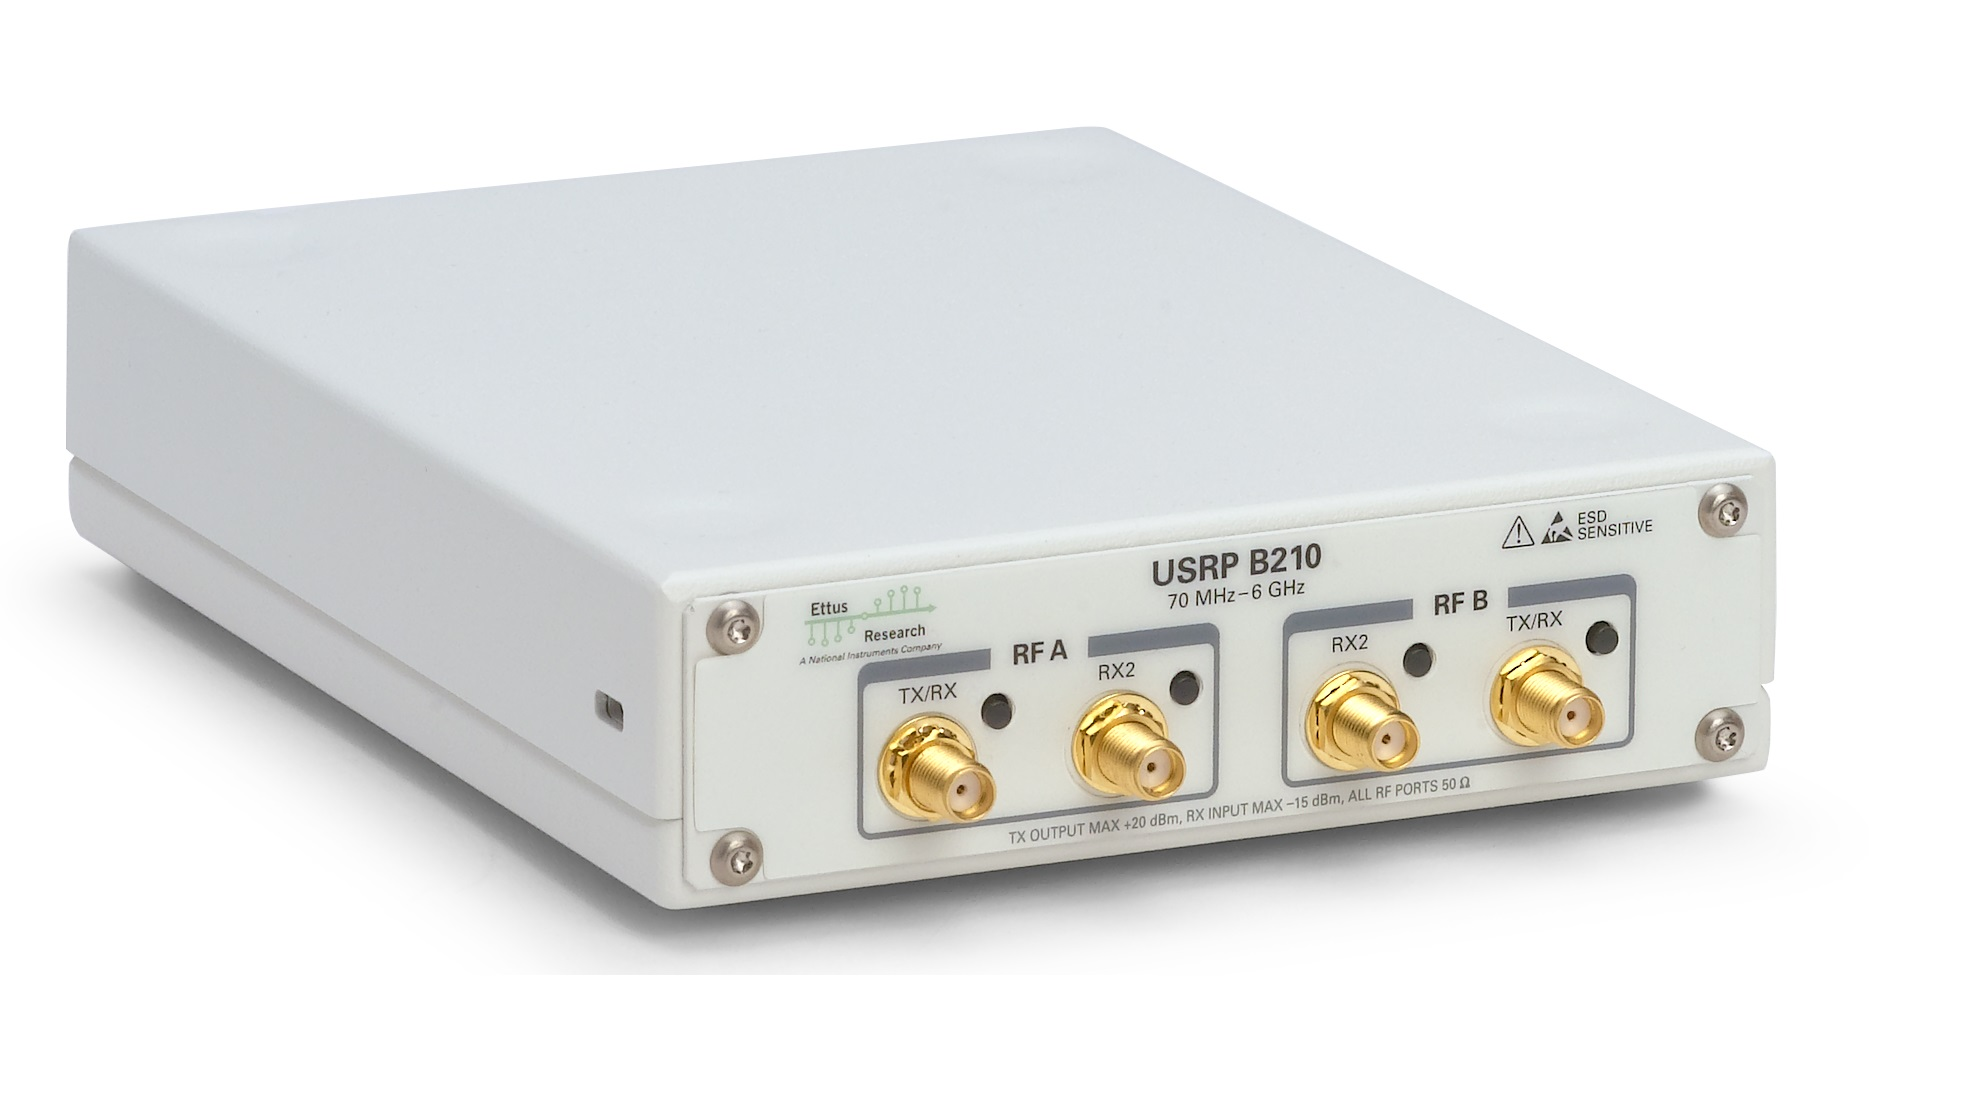
\includegraphics[width=\linewidth]{pics/bab2/B210.jpg}
			\caption{USRP B210 dengan \textit{enclosure}}
		\end{subfigure}
		\begin{subfigure}[b]{0.5\linewidth}
			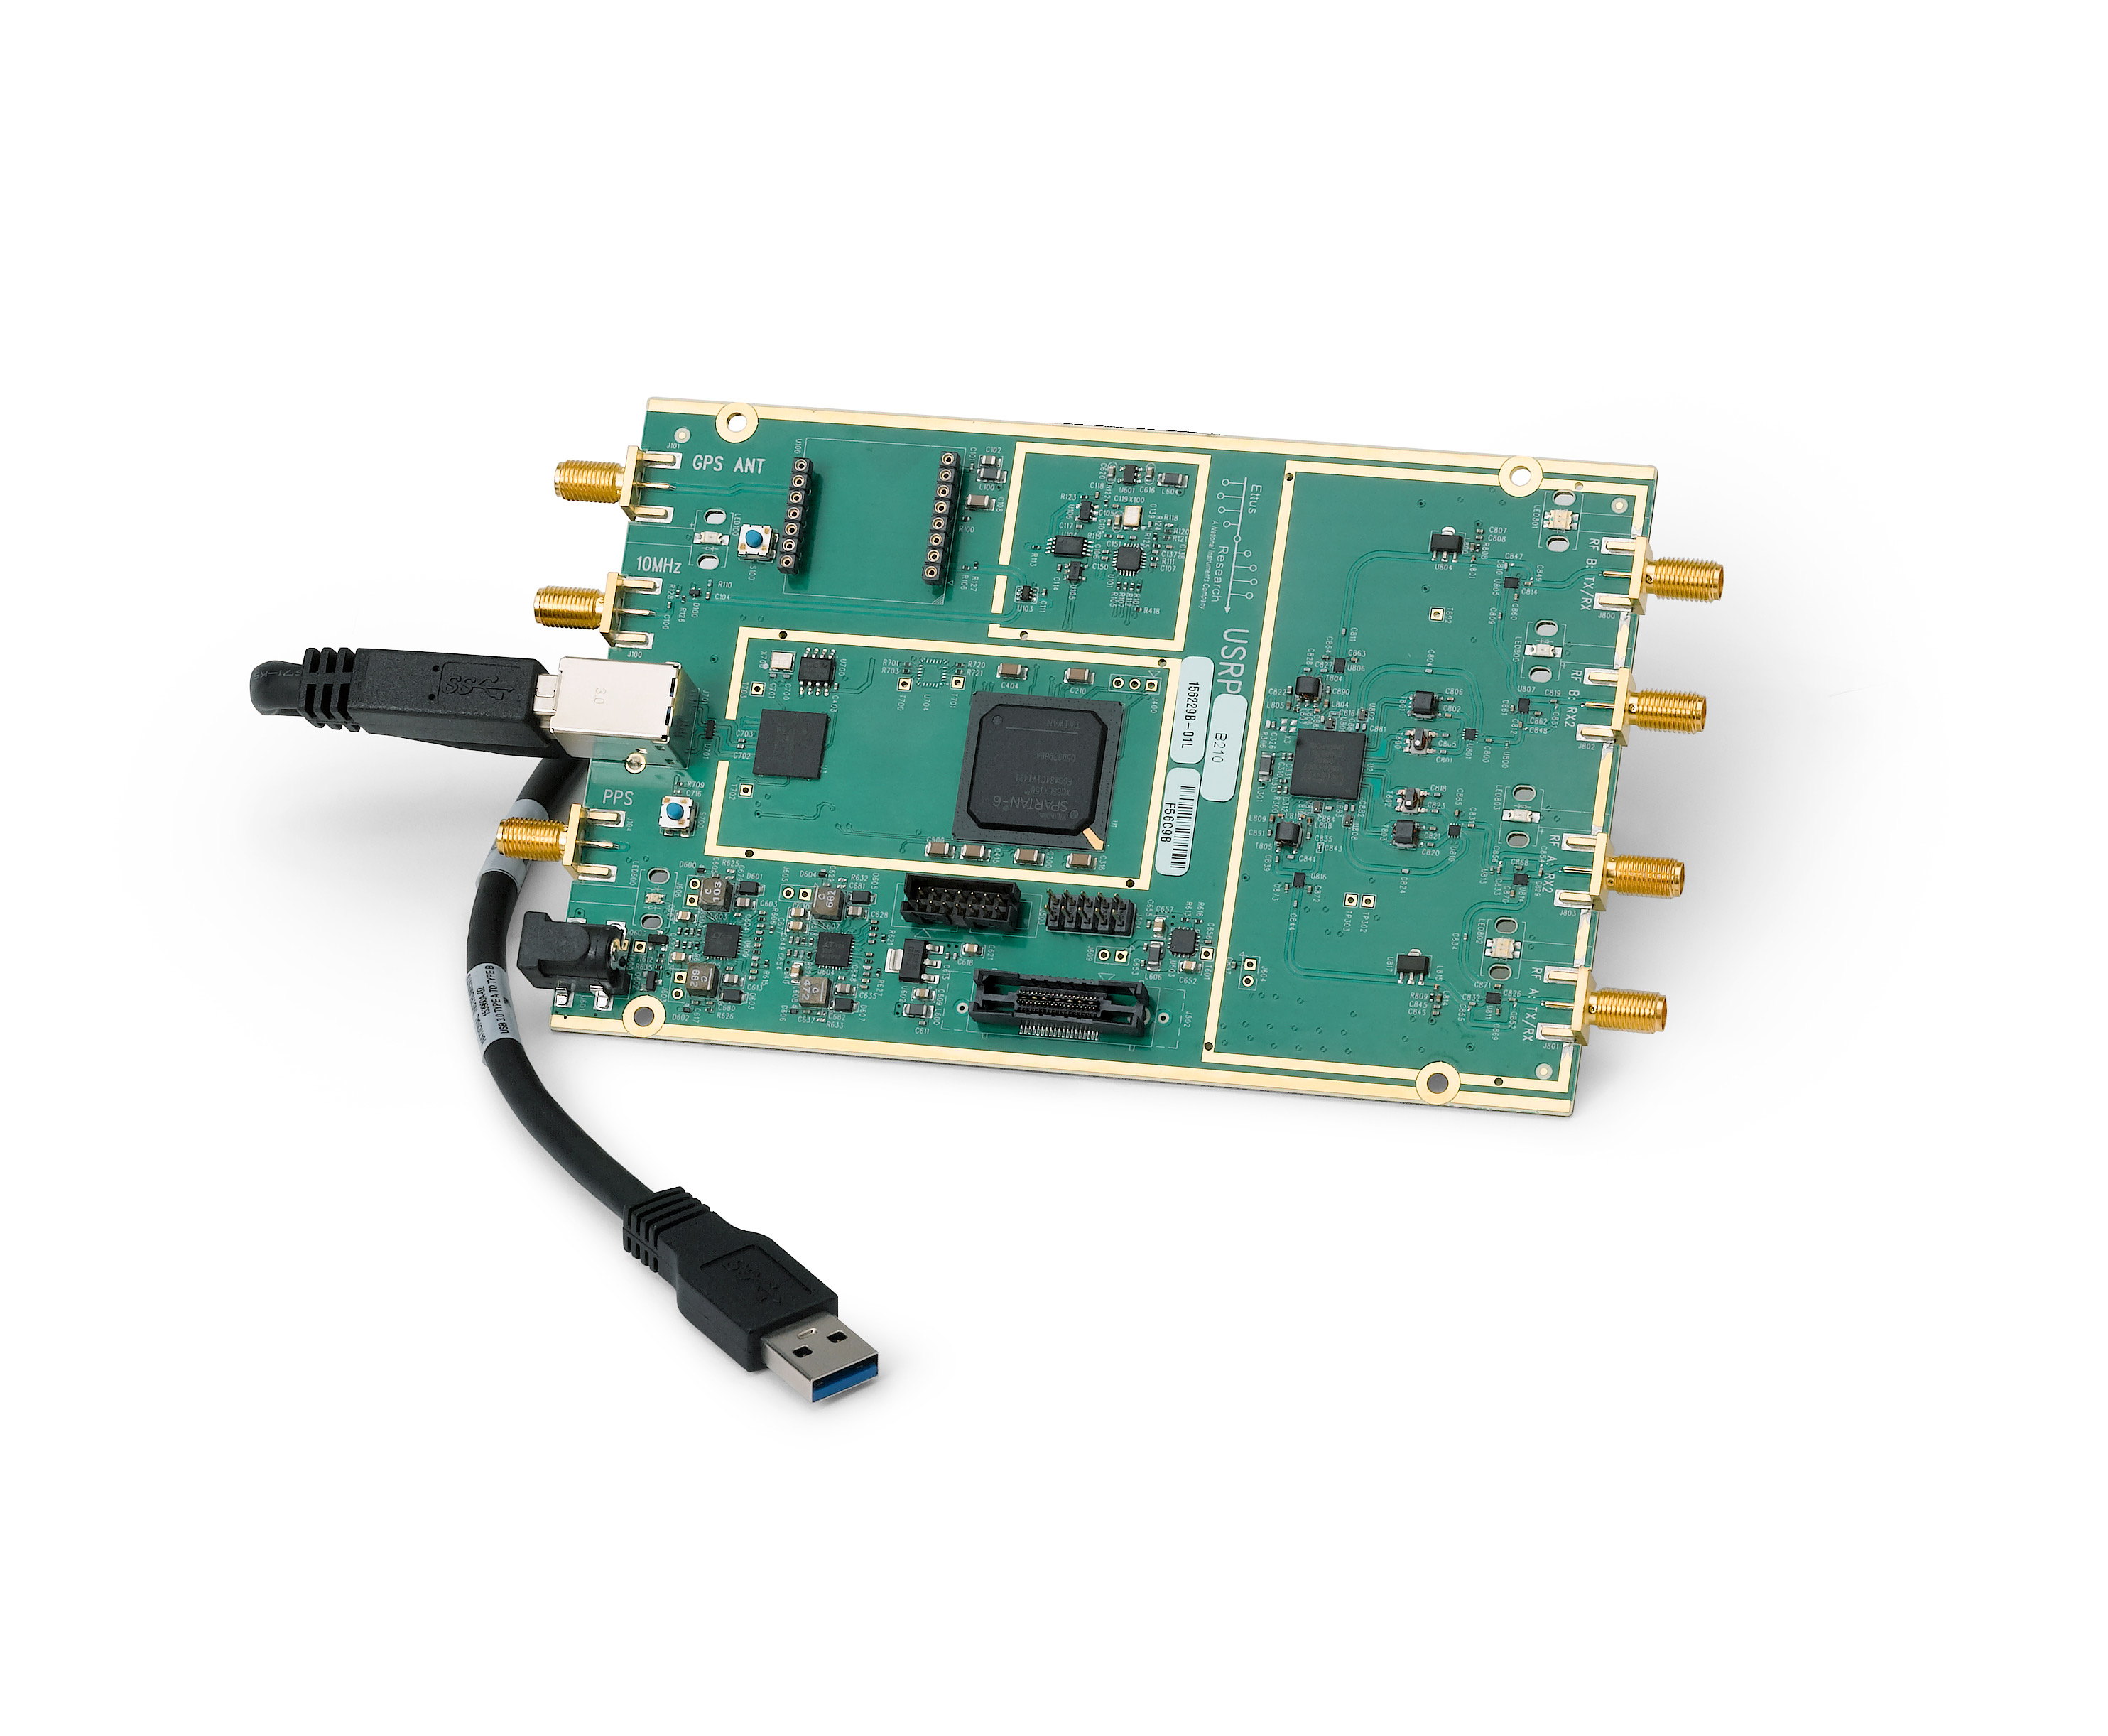
\includegraphics[width=\linewidth]{pics/bab2/B210Board.jpg}
			\caption{\textit{Board} USRP B210}
		\end{subfigure}
		\caption{USRP B210}
		\label{pic:gambarusrp}
	\end{figure}
\end{center}


Kemampuannya untuk berinteraksi dengan gelombang radio inilah, ditambah dengan kemudahannya untuk melakukan pemrograman terhadap USRP yang membuat alat ini terkenal di kalangan akademisi dan peneliti. Karena pengembangan prototipe menjadi lebih mudah tanpa perlu pengadaan komponen.

Ada beberapa USRP di pasaran, salah satunya adalah USRP buatan dari \textit{Ettus} dengan seri B210 seperti pada gambar \ref{pic:gambarusrp}. Penggunaan seri ini dikarenakan seperti yang dapat dilihat pada tabel spesifikasi \ref{tab:spekb210}, USRP ini cukup memenuhi kebutuhan riset dengan kapabilitas pengolahan sampel yang baik.

\begin{longtable}{|c|c|c|c|}
	\caption{Spesifikasi \textit{USRP} B210}
	\label{tab:spekb210}\\
	\hline
	No. & Keterangan & Nilai & Satuan \\
	\hline
	1. & \textit{RF Coverage} & 70 - 6 & MHz - GHz \\
	\hline
	2. & \textit{Analog to Digital Converter Sample Rate} (maksimum) & 61.44 & MS/s \\
	\hline
	3. & \textit{Analog to Digital Resolution}  & 12 & bits	\\
	\hline
	4. &\textit{Analog to Digital Wideband SFDR} & 78 & dBc \\
	\hline
	5. & \textit{Digital to Analog Converter Sample Rate} (maksimum) & 61.44 & MS/s \\
	\hline
	6. & \textit{Digital to Analog Resolution}  & 12 & bits	\\
	\hline
	7. & \textit{Host Sample Rate} (16b) & 61.44 & MS/s \\
	\hline
	8. & \textit{Frequency Accuracy} & $\pm 2.0$ & ppm \\
	\hline
	9. &  \textit{W/ GPS Unlocked TCXO Reference} & $\pm 75$ & ppb \\
	\hline
	10. & \textit{W/ GPS Locked TCXO Reference} & $<$ 1 & ppb \\ 
	\hline
\end{longtable}

Dengan spesifikasi tersebut, maka USRP B210 memiliki kemampuan \textit{instantneous bandwidth} hingga 56 MHz pada transmisi 1 X 1 dan 30.72 MHz pada transmisi 2 X 2.

\subsection{\textit{GNURadio}}

\begin{figure}
	\begin{center}
		
\includegraphics[scale=0.35]{pics/bab2/GNU.png} 
		\caption[Logo GNURadio]{Logo GNURadio}
		\label{pic:logoGnuRadio}
	\end{center}
\end{figure}
GNURadio adalah aplikasi yang dapat melakukan pemrograman terhadap USRP lewat antarmuka. GNURadio merupakan \textit{software open source} sehingga semua orang dapat mengakses, mengubah, dan membagikan \textit{source code} dari program tersebut secara bebas. Dengan menggunakan aplikasi ini, perubahan parameter pada USRP dapat dilakukan dengan mudah.

\begin{figure}
	\begin{center}
		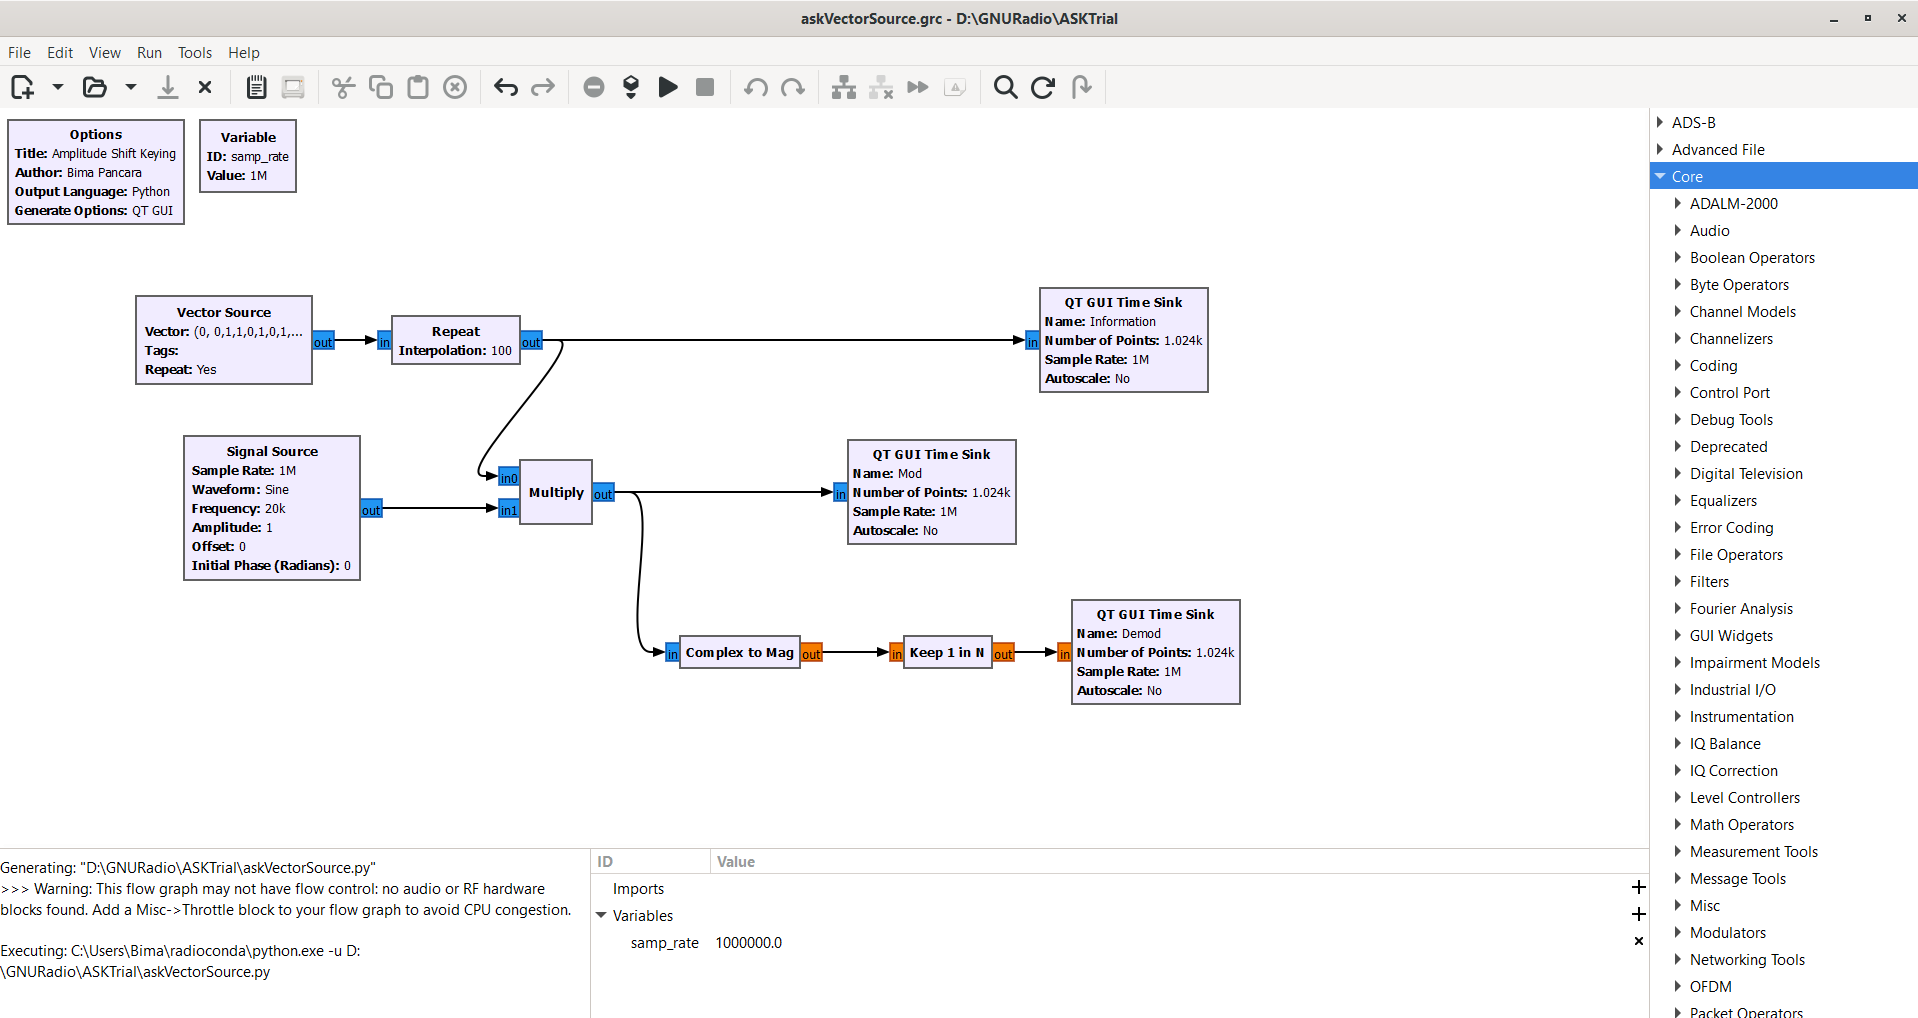
\includegraphics[scale=0.3]{pics/bab2/blokDiagramGRC.png} 
		\caption[Contoh \textit{Flowgraph} GNURadio]{Contoh \textit{Flowgraph} GNURadio}
		\label{pic:contohFlowGraphGRC}
	\end{center}
\end{figure}

Gambar \ref{pic:contohFlowGraphGRC} adalah contoh blok diagram sistem (\textit{flowgraph}) yang sukses dibuat pada aplikasi GNURadio. Pada gambar \ref{pic:contohRunGRC} menunjukkan hasil bila desain sistem tersebut dijalankan.

\begin{figure}
	\begin{center}
		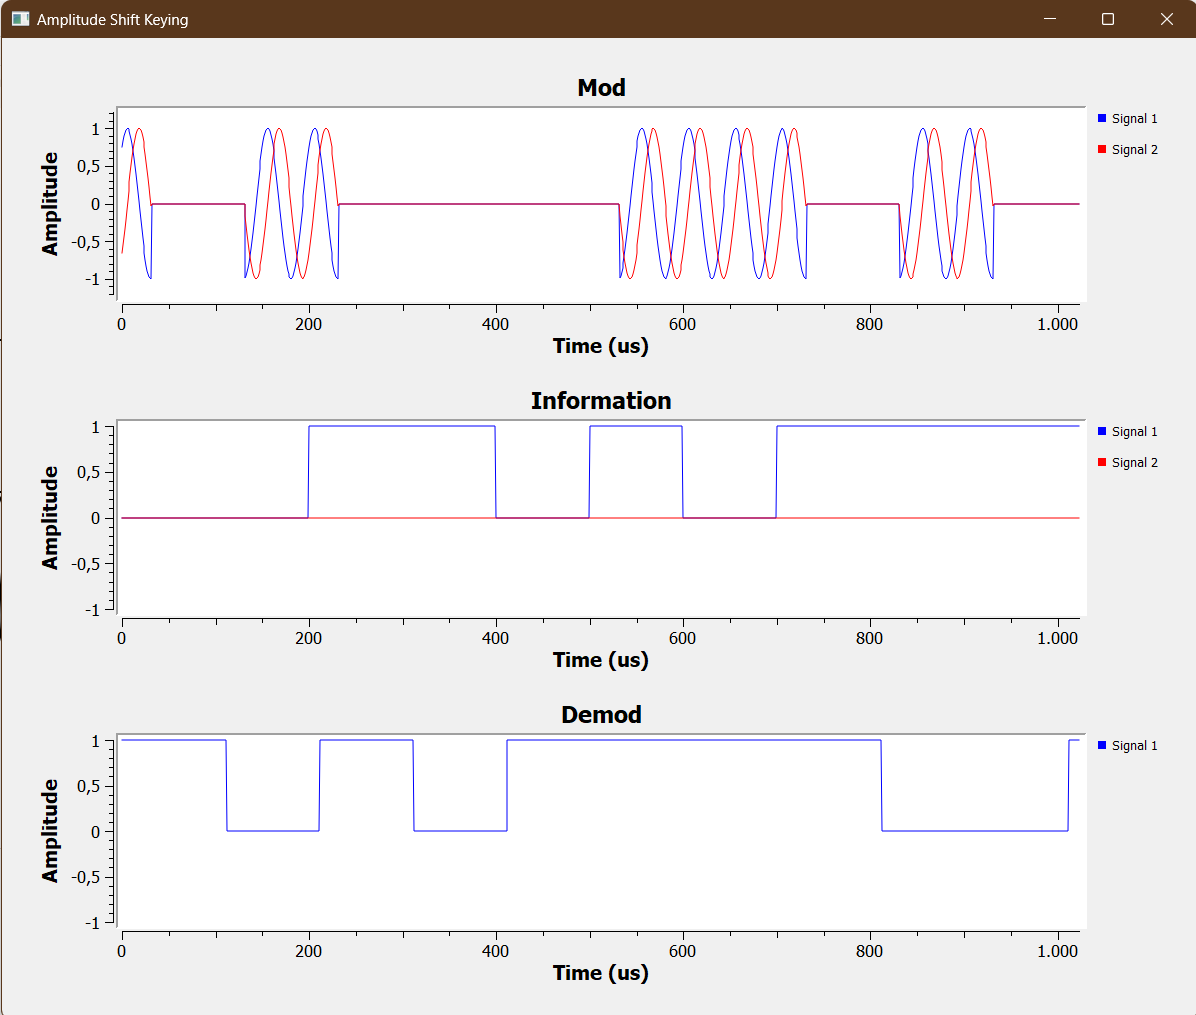
\includegraphics[scale=0.4]{pics/bab2/contohRunGRC.png} 
		\caption[Contoh Hasil Desain Sistem GNURadio]{Contoh Hasil Desain Sistem GNURadio}
		\label{pic:contohRunGRC}
	\end{center}
\end{figure}



